\documentclass[12pt,a4paper]{article}

\usepackage{polski}
\usepackage[utf8]{inputenc}
\usepackage{indentfirst} 

\usepackage{fancyhdr}
\usepackage{graphicx} 
\usepackage[obeyspaces]{url}
\usepackage{lastpage}

\graphicspath{ {./resources/} }

\pagestyle{fancy}
\fancyhf[]{}
\linespread{1.5}
\setlength\headheight{14.5pt}
\cfoot{Strona \thepage \hspace{1pt} z \pageref{LastPage}}
\renewcommand\contentsname{}
\chead{Bieszczadzki Tour --- specyfikacja implementacyjna --- Maciej Czarkowski}

\begin{document}

\begin{titlepage}
\vspace*{\fill}
\begin{center}
{\fontsize{50}{0.1}\selectfont Bieszczadzki Tour}
\huge Specyfikacja implementacyjna
\end{center}
\vspace*{\fill}
\begin{center}
Maciej Czarkowski, 18.11.2019
\end{center}
\end{titlepage}
\clearpage
\hspace{1cm}
\begin{center}
\LARGE\textbf{Spis treści}
\end{center}
\tableofcontents
\clearpage
\section{Wstęp}
Niniejszy dokument, będący specyfikacją implementacyjną projektu \textsl{,,Bieszczadzki Tour''}, ma za zadanie możliwie najlepiej przybliżyć, osobom odpowiedzialnym za jego implementację, sposoby oraz metody prowadzące do stworzenia wydajnego i poprawnie działającego kodu. Program ma rozwiązywać problem odnalezienia optymalnej ścieżki pomiędzy zestawem zadanych punktów, w taki sposób, aby trasa była najkrótsza oraz możliwie najtańsza. Zgodnie z informacjami zawartymi w specyfikacji funkcjonalnej projektu, program do działania wykorzystuje pliki wejściowe, których konfiguracja powinna być zgodna z wyżej wymienionym dokumentem. Pożądanym efektem działania programu jest plik wynikowy, informujący użytkownika, którą trasą się udać, aby droga była optymalna.\\
\section{Środowisko deweloperskie}
Implementacja programu będzie odbywała się na komputerze \textsl{Dell Vostro 3578}, z 4-rdzeniowym procesorem \textsl{Intel Core i5-8250U}, korzystającym z~systemu \textsl{Windows 10 Pro} w wersji 64-bitowej \textsl{10.0.18362}. Program zaimplementowany będzie w języku \textsl{Java} w wersji 8. Implementacja będzie odbywała się w środowisku programistycznym \textsl{IntelliJ IDEA 2018.3 (Community Edition)
Build \#IC-183.4284.148}, wydanym 21 listopada 2018 roku, z wykorzystaniem narzędzi deweloperskich z pakietu \textsl{OpenJDK 64-Bit Server VM by JetBrains s.r.o Windows 10 10.0}. Środowiskiem uruchomieniowym dla kodu będzie maszyna wirtualna Javy w wersji \textsl{1.8.0\_152-release-1343-b15 amd64}.
\section{Zasady wersjonowania}
\subsection{Współpraca z systemem kontroli wersji}
Projekt będzie przechowywany na zdalnym repozytorium, przygotowanym do realizacji projektu indywidualnego z Algorytmów i Struktur Danych. Kolejne funkcjonalności będą realizowane na osobnych gałęziach, po czym, po ich pełnym wykonaniu, będą scalane z gałęzią \textsl{master} repozytorium.
\subsection{Schemat wiadomości}
Każda aktualizacja zawartości repozytorium (\textsl{commit}), która będzie przekazywana na odpowiednią gałąź w repozytorium, będzie opatrzona odpowiednią wiadomością, zgodną ze schematem dotyczącym pierwszego słowa w~wiadomości, które identyfikowało będzie poczynioną w kodzie modyfikację:
\begin{itemize}
\item ,,\path{add}'' w przypadku dodania nowego elementu do kodu;
\item ,,\path{delete}'' w przypadku usunięcia określonego fragmentu kodu;
\item ,,\path{fix}'' w przypadku naprawiania niedziałających segmentów kodu;
\item ,,\path{modify}'' w przypadku drobnych modyfikacji w kodzie;
\item ,,\path{refactor}'' w przypadku znaczących zmian w kodzie, dotyczących większego fragmentu kodu;
\item ,,\path{approve v. x.x.}'', gdzie x.x. to wartości od 0.1 do 1.0 (wersji ostatecznej), w przypadku zatwierdzenia kolejnej wersji do wydania --- dodania na gałąź master.
\end{itemize}
\section{Diagram klas i struktura programu}
Niniejszy rozdział opisuje strukturę programu, wyróżniając kolejne wykorzystywane klasy.
\subsection{DataReader}
Jest to klasa odpowiedzialna za walidację danych wejściowych do programu. Analizuje ona otrzymane argumenty, a jeśli którykolwiek z nich nie jest zgodny z przyjętym formatem, informuje użytkownika o błędzie. Zczytane z pliku wejściowego miejsca zostaną umieszczone na liście, po czym po zakończeniu jej wypełniania utworzona zostanie tablica, która przechowywała będzie czasy przejść pomiędzy miejscami. Dzięki metodzie \textsl{fillTimesVector} ID miejsc są konwertowane na unikalną wartość liczbową, która będzie identyfikowała dane miejsce w programie.
\subsection{Map}
Jest to klasa reprezentująca strukturę mapy punktów, które rozważamy przy tworzeniu optymalnej ścieżki. Mapa punktów przedstawiona jest w postaci tablicy dwuwymiarowej przechowującej czasy przejść pomiędzy miejscami na mapie.
\subsection{Place}
Klasa ta zawiera model pojedynczego elementu mapy. Atrybutami tej klasy są ID miejsca, pełna jego nazwa oraz numeryczne, unikalne ID, niezbędne, aby można było identyfikować punkty w tablicy czasów przejść.
\subsection{MainAlgorithm}
Jest to klasa realizująca główną logikę programu. W przypadku pojawienia się na wejściu pliku \path{wishlist} klasa ta przekazuje mapę miejsc do modyfikacji metodom z klasy \textsl{DijkstraAlgorithm}.
Metoda \textsl{calculateWholePath} zwraca tablicę numerycznych ID miejsc w kolejności, w której powinny one zostać odwiedzone.
\subsection{DijkstraAlgorithm}
Klasa tworząca, na podstawie otrzymanej mapy punktów i czasów przejść pomiędzy nimi, nową mapę, uwzględniającą jedynie miejsca, które pojawiły się w pliku \path{wishlist}. Wykorzystuje ona algorytm Dijkstry, który pozwala znaleźć najkrótsze możliwe ścieżki w grafie pomiędzy dwoma węzłami.
\subsection{DataWriter}
Klasa wypisująca otrzymany rezultat działania algorytmu do pliku wynikowego \path{result.txt}. Na podstawie otrzymanego od klasy MainAlgorithm wektora, klasa odtwarza nazwy miejsc i wypisuje je do pliku wyjściowego.
\begin{figure}[h!]
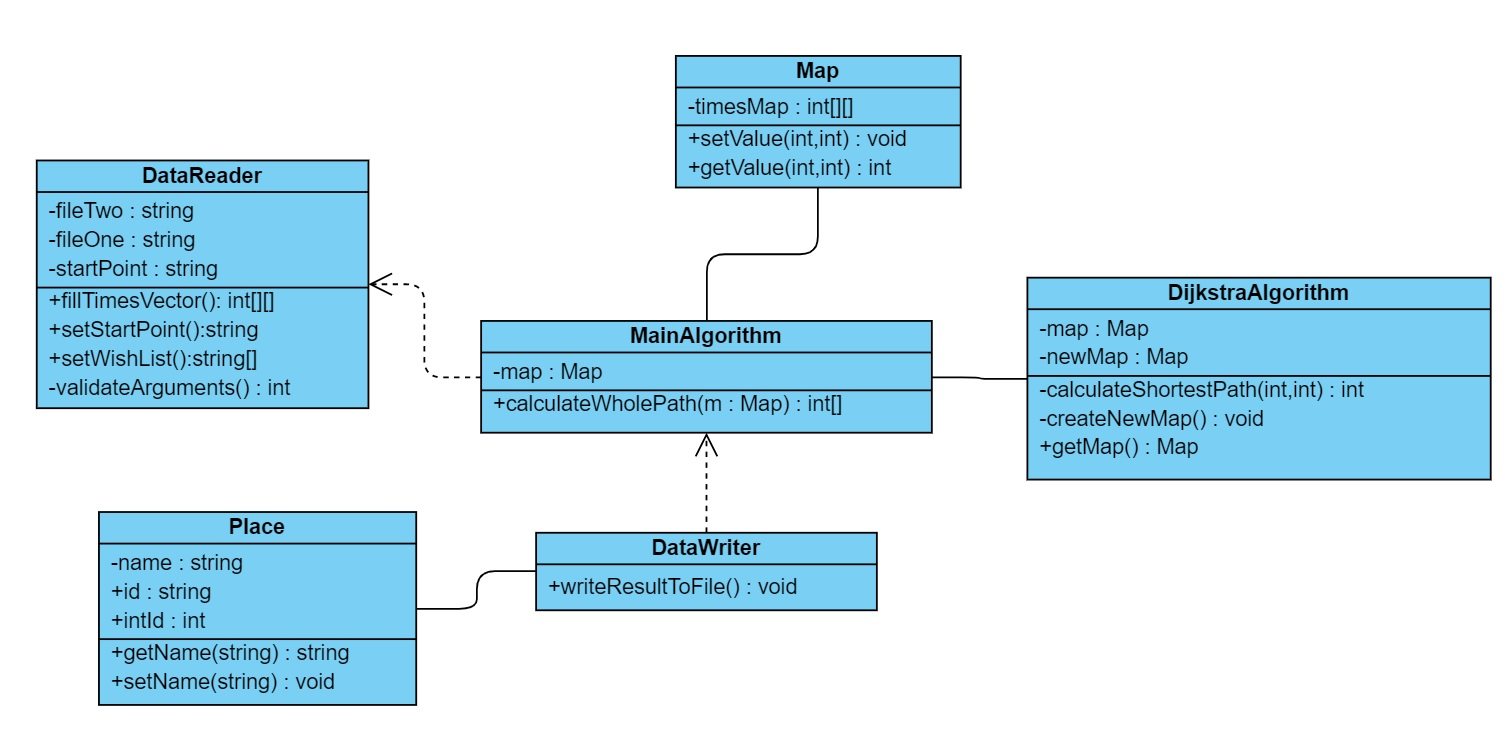
\includegraphics[width=\linewidth]{ClassDiagram.jpg}
\caption{Diagram klas programu}
\end{figure}
\newpage
\section{Rozwiązywany problem}
Rozwiązywanym przez program problemem jest zagadnienie optymalizacyjne polegające na znalezieniu cyklu zamkniętego w grafie ważonym o~~możliwie najmniejszym koszcie, nazywane \textsl{Problemem komiwojażera}. Jest to algorytm NP-trudny, charakteryzujący się dużą złożonością obliczeniową przy kierowaniu się metodą \textsl{brute force} --- przy sprawdzaniu wszystkich możliwych połączeń pomiędzy wszystkimi węzłami otrzymujemy złożoność obliczeniową rzędu n!, co już przy niewielu węzłach (20) powoduje praktyczny brak możliwość realizacji programu poprzez niezwykle długi czas wykonania. W~tej~~sytuacji, stosownym rozwiązaniem jest zastosowanie algorytmów przybliżających optymalną trasę, jednakże działających w możliwym do zaakceptowania czasie.
\section{Wykorzystane algorytmy}
Program opiera się na wykorzystaniu algorytmu Dijkstry oraz algorytmu najbliższego sąsiada. Pierwszy z wymienionych algorytmów wykorzystany zostanie przy tworzeniu pomniejszonej mapy punktów, które chcemy odwiedzić. Odnajduje on najkrótszą możliwą ścieżkę pomiędzy dwoma określonymi węzłami w grafie. Algorytm najbliższego sąsiada pozwoli odnaleźć estymowaną optymalną trasę pomiędzy wybranymi punktami, bądź pomiędzy wszystkimi, jeśli plik \path{wishlist} nie został podany jako argument. Jest to algorytm zachłanny, wybierający jako ścieżki przejścia pomiędzy węzłami ścieżki o możliwie najmniejszej wadze, jednakże biorąc pod uwagę, że rozwiązywany problem jest NP-trudny, taki algorytm zagwarantuje wystarczająco przybliżone rozwiązania do optymalnego --- wyznaczone ścieżki powinny być maksymalnie 25\% gorsze od optymalnej. Dla tego algorytmu złożoność obliczeniowa to~~$n^2$, co czyni go wartym wykorzystania.
\section{Istotne struktury danych}
Główną strukturą danych, którą będzie wykorzystywał program jest dwuwymiarowa tablica wartości całkowitych, identyfikująca czasy przejść w minutach pomiędzy poszczególnymi miejscami. Wykorzystana zostanie również lista liniowa, która pozwoli na wejściu programu zebrać wszystkie dane, które następnie zostaną wpisane odpowiednio do tablicy czasów przejść.
\end{document}

